%!TEX program = xelatex

\documentclass[compress]{beamer}
%--------------------------------------------------------------------------
% Common packages
%--------------------------------------------------------------------------

\definecolor{links}{HTML}{663000}
\hypersetup{colorlinks,linkcolor=,urlcolor=links}

\usepackage[english]{babel}
\usepackage{pgfpages} % required for notes on second screen
\usepackage{graphicx}

\usepackage{multicol}


\usepackage{tabularx,ragged2e}
\usepackage{booktabs}

\setlength{\emergencystretch}{3em}  % prevent overfull lines
\providecommand{\tightlist}{%
  \setlength{\itemsep}{0pt}\setlength{\parskip}{0pt}}


\usetheme{hri}

\usepackage{remreset}% tiny package containing just the \@removefromreset command
\makeatletter
\@removefromreset{subsection}{section}
\makeatother
\setcounter{subsection}{1}

\newcommand{\source}[2]{{\tiny\it Source: \href{#1}{#2}}}

\usepackage{tikz}
\usetikzlibrary{mindmap,backgrounds,positioning}

\graphicspath{{figs/}}

\title{ROCO318 \newline Mobile and Humanoid Robots}
\subtitle{Part 1 -- Introduction}
\date{}
\author{Séverin Lemaignan}
\institute{Centre for Neural Systems and Robotics\\{\bf Plymouth University}}

\begin{document}

\licenseframe{github.com/severin-lemaignan/module-mobile-and-humanoid-robots}

\maketitle

\imageframe[color=black, caption=github.com/severin-lemaignan/module-mobile-and-humanoid-robots]{github}

\imageframe[scale=1]{pepper-robot}

\section{What have we seen so far?}

\begin{frame}[plain]

    \begin{multicols}{2}

        \begin{center}
            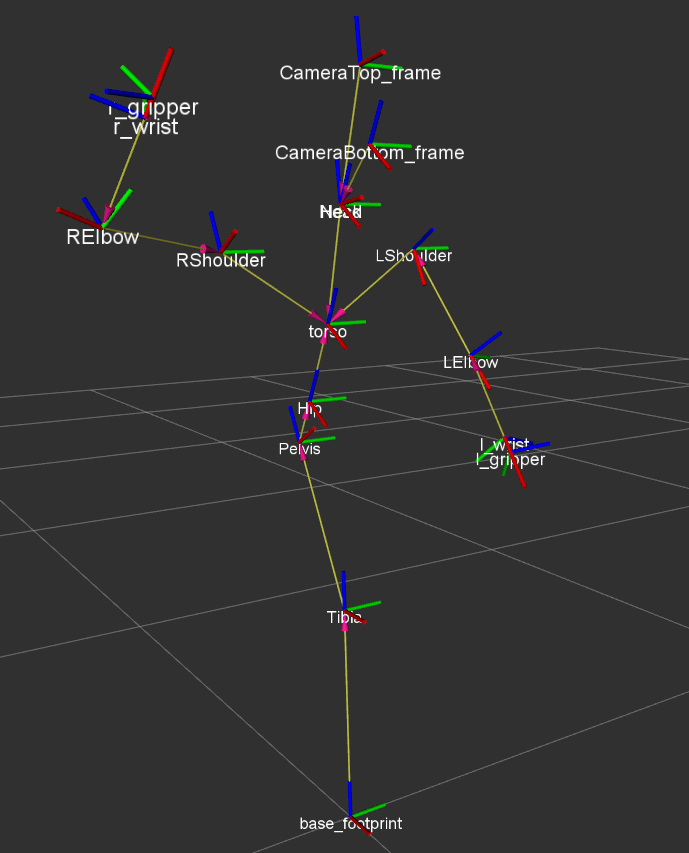
\includegraphics[width=\linewidth]{frames_pepper}
        \end{center}
        \vfill\columnbreak

        \begin{itemize}
            \item \textbf{frames}
            \item \textbf{forward kinematics}
            \item \textbf{inverse kinematics}
        \end{itemize}

    \end{multicols}
\end{frame}

\begin{frame}[plain]

    \begin{center}

        \textbf{Lots of sensors!}

        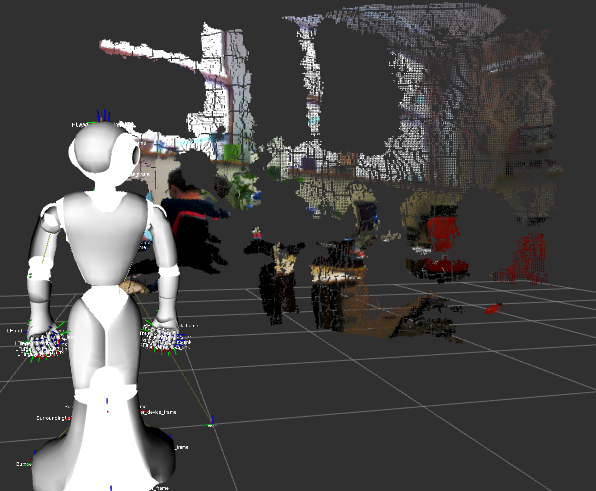
\includegraphics[width=0.6\linewidth]{rgbd_pepper}

    \end{center}

        \begin{itemize}
            \item \textbf{RGB-D cameras}, color + depth registration
            \item \textbf{Laserscans}
            \item \textbf{Sonars},...
        \end{itemize}

\end{frame}

\imageframe[color=black,caption=2D mapping!]{mapping_pepper}
\imageframe[color=black, caption=3D mapping!]{octomap_pepper}

\begin{frame}[plain]

    \begin{center}

        \textbf{Odometry is not good enough}

        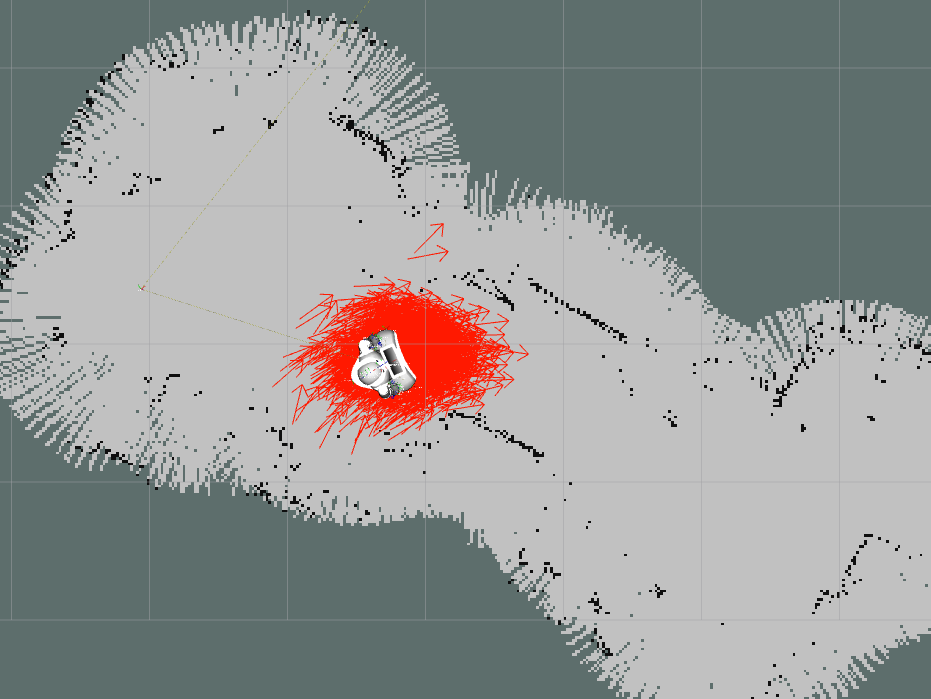
\includegraphics[width=0.6\linewidth]{localisation_pepper}

    \end{center}

        \begin{itemize}
            \item \textbf{SLAM} (Simultaneous Localization and Mapping)
            \item using \textbf{probabilistic reasoning} (Monte-Carlo localisation)
        \end{itemize}

\end{frame}

\imageframe[color=black,caption=Costmaps \& Motion planning]{motion_planning_pepper_rviz}

\begin{frame}[plain]

\begin{center}
    \textbf{Robotic middleware} to connects components together
    \vspace{3em}

\begin{tikzpicture}[
                    >=latex,
                    every edge/.style={->, draw, very thick},
                    service/.style={->, draw, very thick,dashed},
                    rosnode/.style={draw, font=\sf, node distance=0.5, rounded
                    corners, align=center, inner sep=5pt,fill=hriSec2Dark!50},
                    topic/.style={font=\tt, node distance=0.5, align=center, inner sep=5pt},
                    pic/.style={fill=none,draw=none}
                ]

    \path[use as bounding box] (-6,1) rectangle (6,-5);
    \node [rosnode] at (0,0) (node1) {node 1};
    \node [rosnode] at (4,-2) (node2) {node 2};
    \node [rosnode] at (-5,-4) (node3) {node 3};

        \node [topic] at (1,-2) (topic1) {/topic1};
        \node [topic] at (-1,-3) (topic2) {/topic2};
        \node [topic] at (-4,-2) (topic3) {/topic3};
        \path (node1) edge[bend left] node[label,right] {} (topic1);
        \path (node1) edge[bend right] node[label,left] {publishes} (topic2);
        \path (node3) edge[bend left] node[label,left] {} (topic3);
        \path (topic1) edge[bend right] node[label,below left] {subscribes} (node2);
        \path (topic2) edge[bend left] node[label,below] {} (node3);
        \path (topic2) edge[bend right] (node2);
        \path[->, dashed] ([yshift=2pt]node1.east) edge[bend left] node[label,above right] {action goal} ([xshift=2pt]node2.north) ;
        \path[->, dashed] ([xshift=-2pt]node2.north) edge[bend right] node[label,below left] {result} ([yshift=-2pt]node1.east);

        \node [rosnode,fill=hriSec3!50] at (-5,0) (roscore) {roscore};
        \path[dashed] (node1) edge[<->,very thin, bend right] node[label,above] {\tiny XML-RPC} (roscore);
        \path[dashed] (node2) edge[<->,very thin, bend right] node[label,above] {\tiny XML-RPC} (roscore);
        \path[dashed] (node3) edge[<->,very thin, bend left] node[label,above right] {\tiny XML-RPC} (roscore);


\end{tikzpicture}
\end{center}

\end{frame}


\begin{frame}[plain]{}
    Well, ROCO318 is over...

    \pause
    (oh no, I forgot about the autonomous chairs...)
\end{frame}


\videoframe[0.56]{figs/NISSAN-ProPILOT-chair.mp4}


\section{Module Overview}
\begin{frame}{This module}

\begin{itemize}
\item Sensors for mobile and humanoid robots
\item Computer vision \emph{(Philip Culverhouse)}
\item Localisation
\item Planning and navigation
\item Bipedal robots
\item Robot control
\end{itemize}

\end{frame}


\begin{frame}{This module}

    How to build intelligent mobile/humanoid robots?\\
    $\neq$ industrial automation!

    \begin{multicols}{2}

        \begin{center}
            
\includegraphics[height=4.5cm]{no-industrial}

            
\includegraphics[height=4.5cm]{yes-humanoid}
        \end{center}

    \end{multicols}

    \pause

    \begin{itemize}
        \item \textbf{Hardware issues}: sensors, actuators, drive mechanisms, \ldots{}
        \item \textbf{Software issues}: robot control, computer vision, learning robots, \ldots{}
    \end{itemize}

\end{frame}

\section{How Widespread?}

\imageframe{industrial-robots-statistics}

\begin{frame}[plain]{}
    But...
\end{frame}

\imageframe{service-robots-stats}


\section{Domains of Robotics}

\begin{frame}{Service/domestic robots}


    \begin{multicols}{2}

        \textbf{Service robots}

        \begin{itemize}
            \item
                iRobot Roomba, 12M units sold.
            \item
                Samsung, LG, Dyson
        \end{itemize}
        \vfill
        \columnbreak

        \begin{center}
            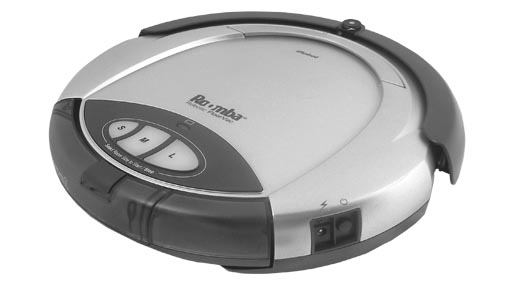
\includegraphics[width=0.5\linewidth]{roomba}
            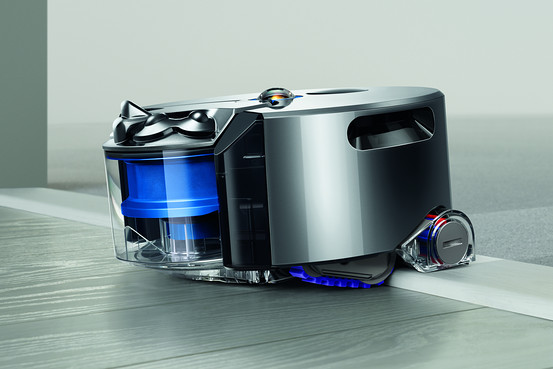
\includegraphics[width=0.5\linewidth]{dyson}
        \end{center}
    \end{multicols}


    \begin{multicols}{2}


        \textbf{Edutainment robots}

        \begin{itemize}
            \item \eg KeepOn, 
            \item Lego Mindstorms (original, NXT, EV3),
            \item RoboSapiens
        \end{itemize}
        \vfill
        \columnbreak
        \begin{center}

            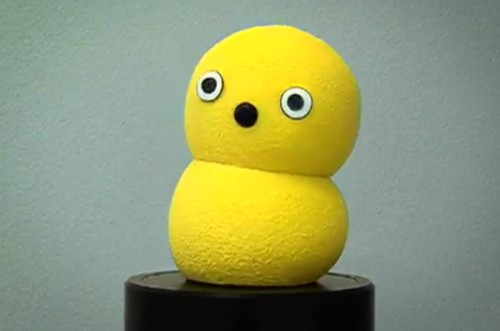
\includegraphics[width=0.6\linewidth]{keepon}

            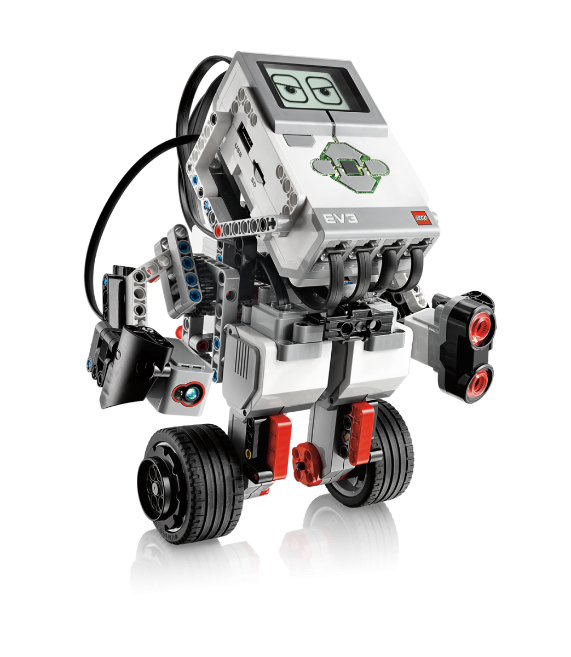
\includegraphics[width=0.5\linewidth]{lego-nxt}
            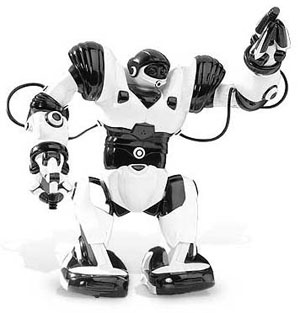
\includegraphics[width=0.5\linewidth]{robosapiens}
        \end{center}
    \end{multicols}
\end{frame}

\begin{frame}{Flying robots}

    \begin{multicols}{2}

Very popular research field and tremendous interest from the military,
some civilian uses (e.g. aerial videoing).

Challenges: autonomy (control of flight parameters), localisation,
energy autonomy, robustness.

    \begin{center}
        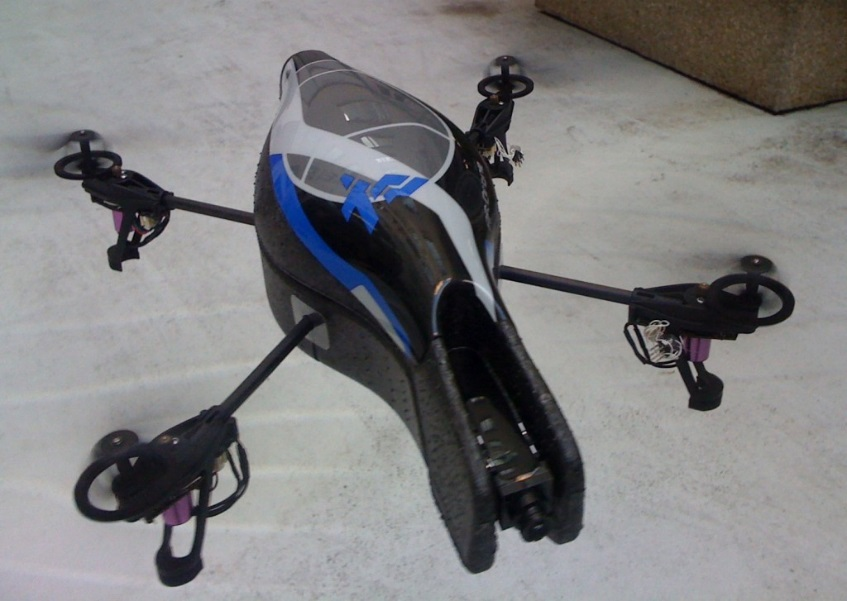
\includegraphics[width=0.8\linewidth]{drone}
    \end{center}

    \end{multicols}
\begin{itemize}
    \item Raffaello D'Andrea's \href{https://www.youtube.com/watch?v=w2itwFJCgFQ}{drone acrobatics}
\item
  \href{http://youtu.be/YQIMGV5vtd4}{U. Pennsylvania, Vijay Kumar's nano
        quadrotors} (see also \href{http://youtu.be/4ErEBkj_3PY}{TED talk})
\item
  EPFL's \href{http://youtu.be/n_qRuHkD5lc}{flying wing robot}.
\end{itemize}

\end{frame}

\begin{frame}{Space exploration}

    \begin{columns}
        \begin{column}{0.6\linewidth}

        Three Mars rovers:

        \begin{itemize}

            \item
                \href{https://en.wikipedia.org/wiki/Sojourner_(rover)}{Sojourner}
                touched down in summer 1997

            \item \href{http://en.wikipedia.org/wiki/Spirit_rover}{Spirit} and
                \href{http://en.wikipedia.org/wiki/Opportunity_rover}{Opportunity}
                landed in January 2004

            \item \href{http://mars.jpl.nasa.gov/msl/mission/overview/}{Curiosity}
                touched down 5 August 2012

        \end{itemize}

        All are fully teleoperated from earth.  However, the sensors
        and software allow for autonomous obstacle detection and
        navigation.

        Have survived 30x longer than planned;
        \href{http://marsrovers.nasa.gov/}{marsrovers.nasa.gov}

        \end{column}

        \begin{column}{0.4\linewidth}
        \begin{center}
            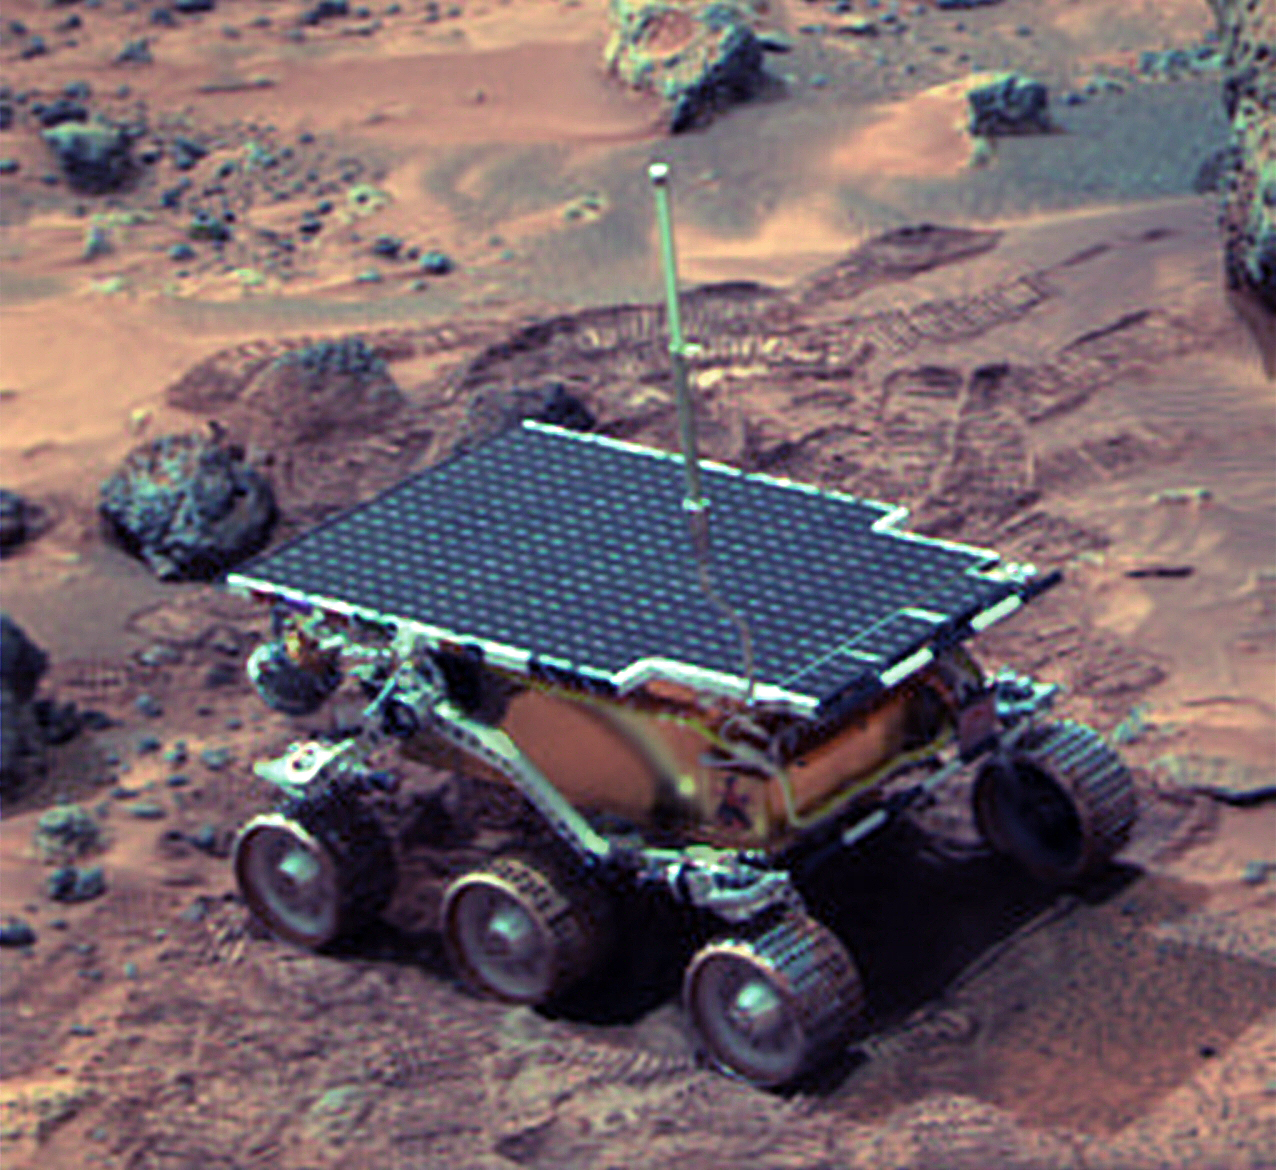
\includegraphics[width=0.6\linewidth]{space-robot-sojourner}

            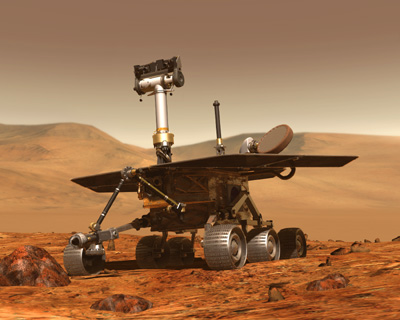
\includegraphics[width=0.6\linewidth]{space-robot-spirit}

            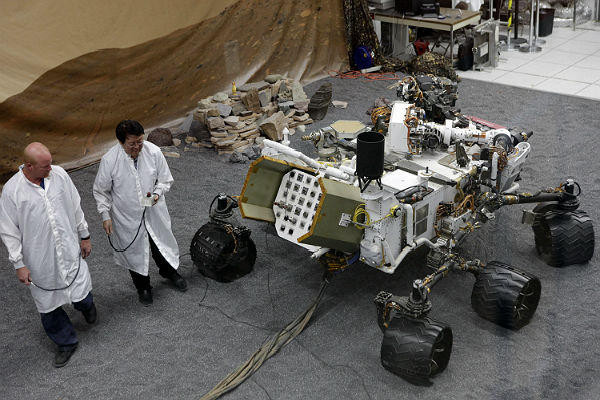
\includegraphics[width=0.6\linewidth]{space-robot-curiosity}
        \end{center}
        \end{column}
    \end{columns}
\end{frame}

\begin{frame}{Military robots}

Best selling ``professional service'' robot: 6500 units in 2011, 6100 in
2012, 9500 in 2013.

    \begin{center}
        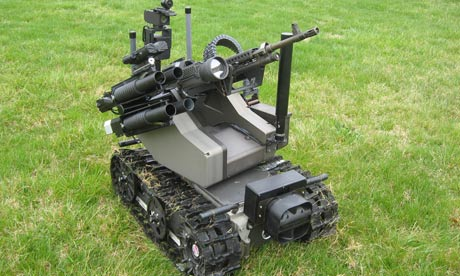
\includegraphics[width=0.6\linewidth]{defence-robot}

        \footnotesize \href{https://en.wikipedia.org/wiki/Modular_Advanced_Armed_Robotic_System}{Modular Advanced Armed Robotic System (MAARS)}
    \end{center}

    Video: \href{http://youtu.be/eaP0waiz43w}{iRobot packbot}

\end{frame}

\begin{frame}{Autonomous cars}

    \centering
    \only<1>{
        \textbf{2005}: Darpa Grand Challenge; $>$200km race in Mojave/Nevada desert

        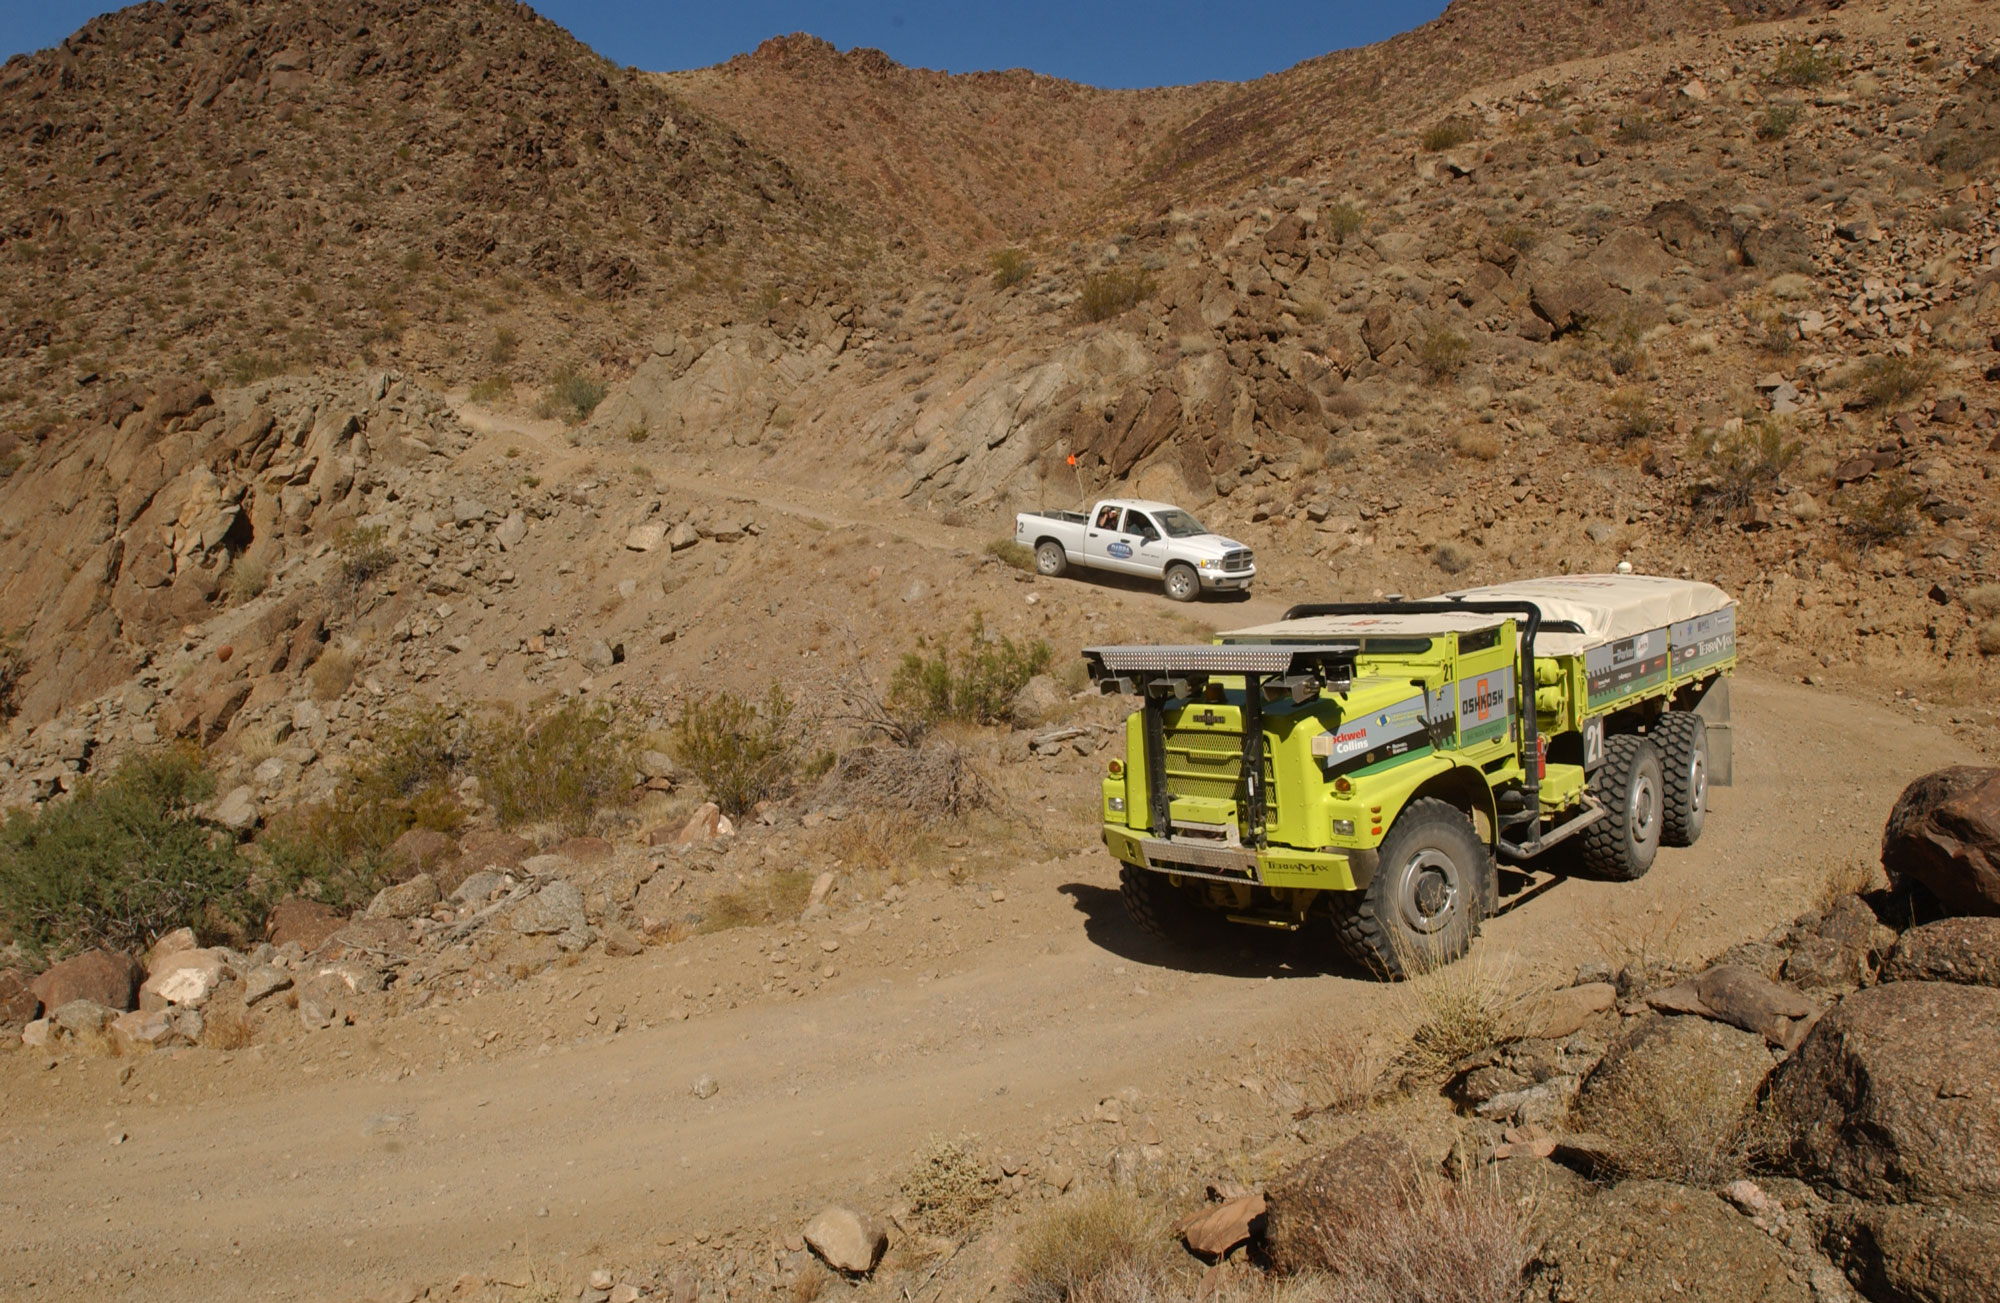
\includegraphics[width=0.8\linewidth]{darpa-grand-challenge}

        \source{https://commons.wikimedia.org/wiki/File:DARPA-2005.jpg}{Wikipedia}
    }
    \only<2>{
        \textbf{2007}: Darpa Urban Challenge; 100km in urban environment, must obey all traffic regulations

        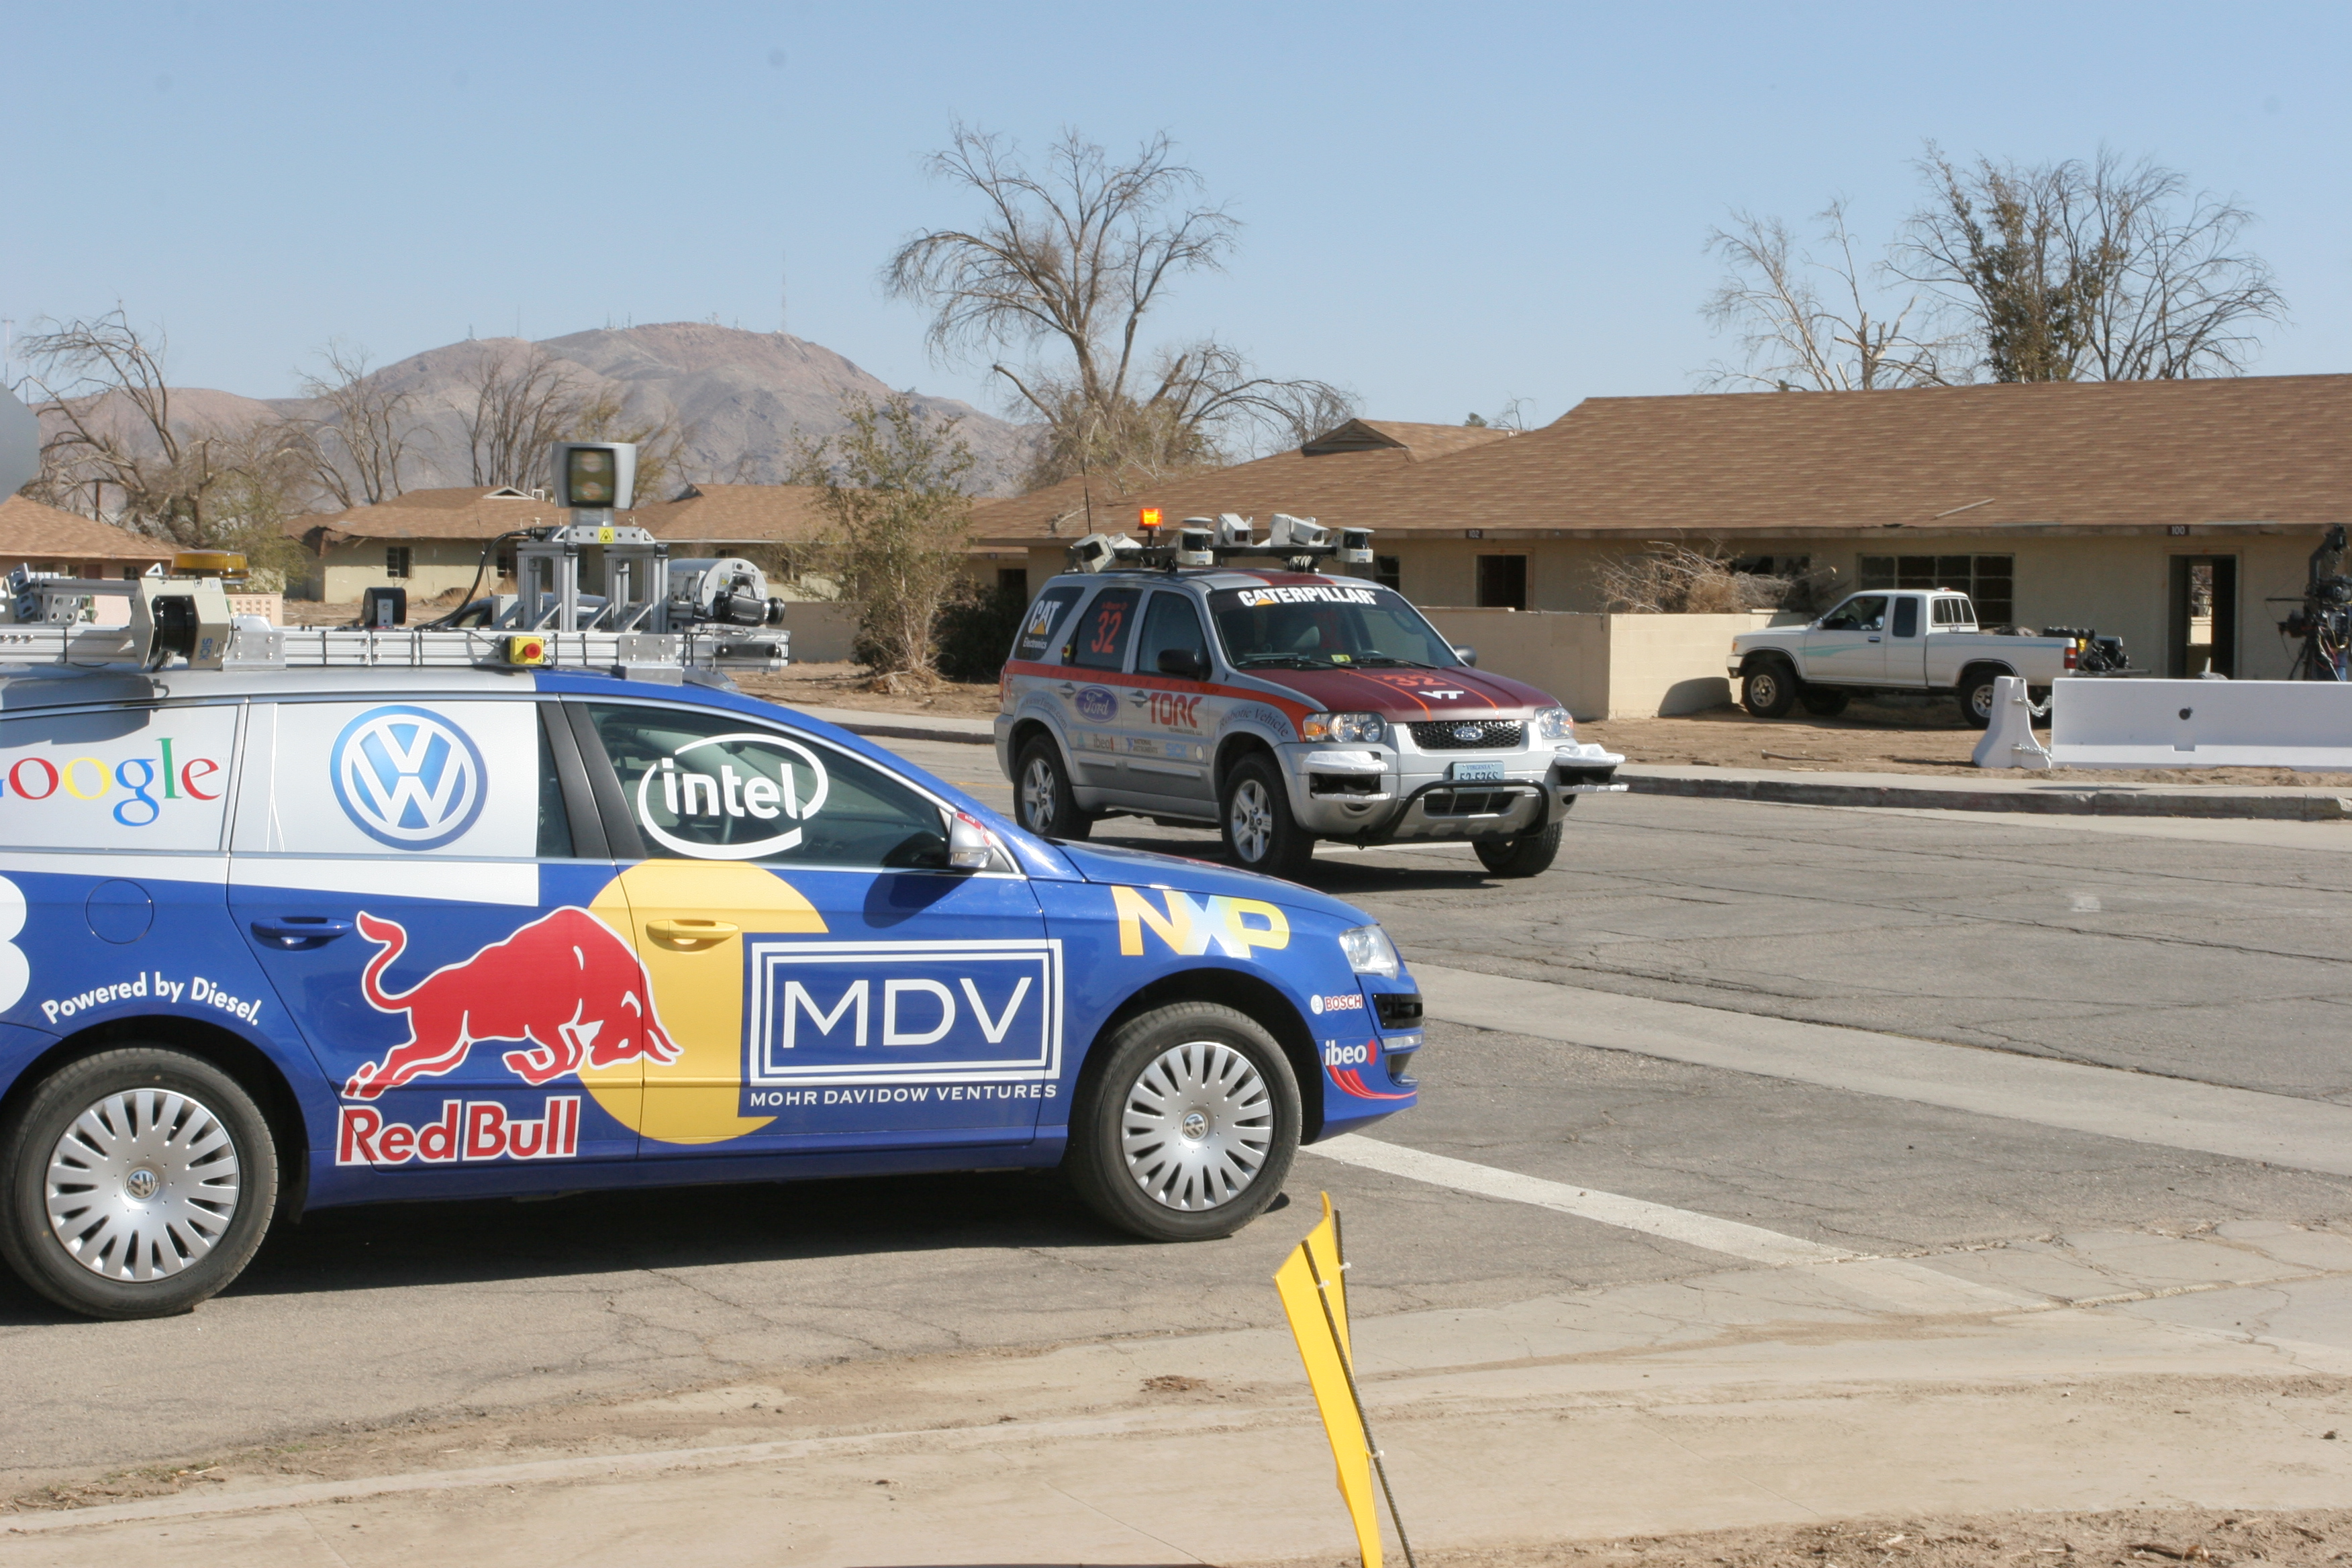
\includegraphics[height=4cm]{darpa-urban-challenge}
        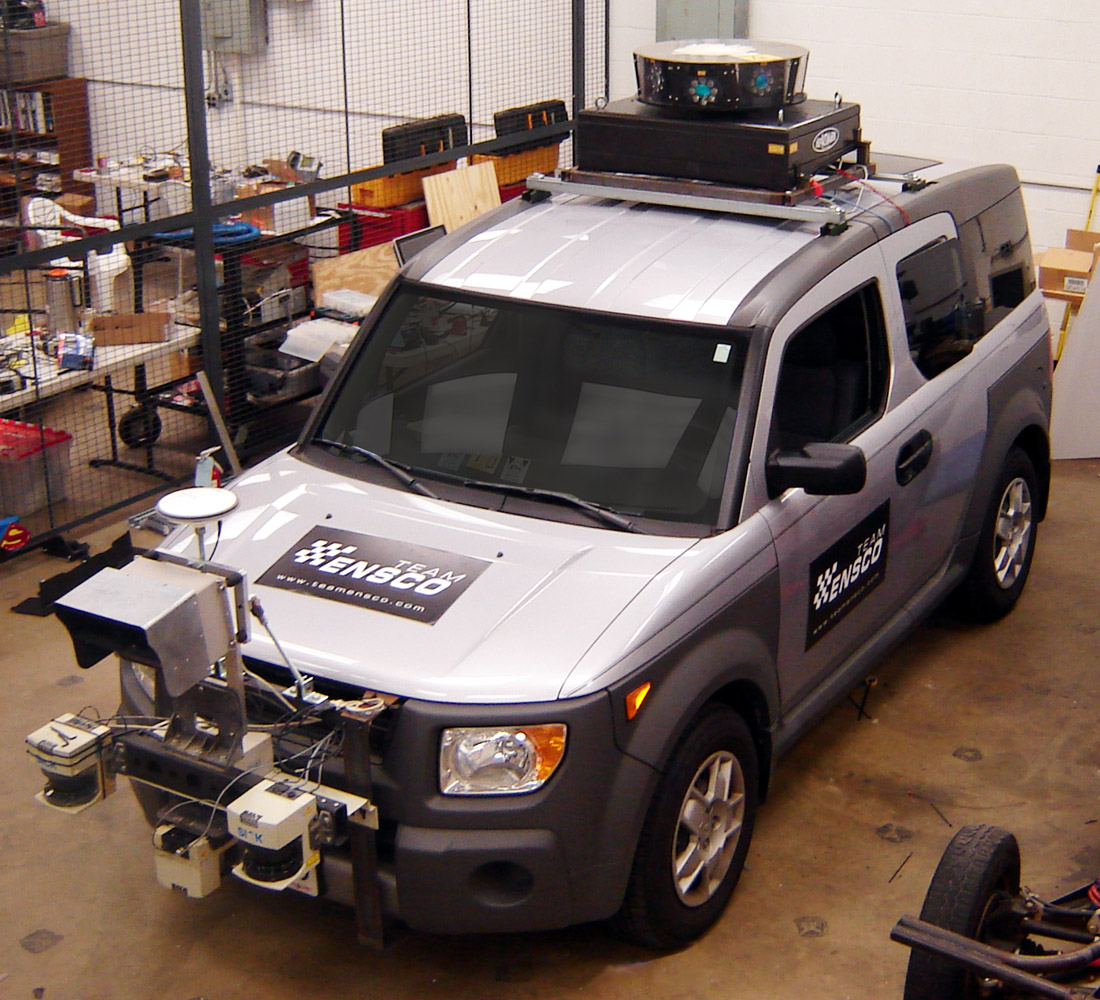
\includegraphics[height=4cm]{darpa-urban-challenge2}

        \source{https://en.wikipedia.org/wiki/File:UrbanChallenge_StandfordRacingandVictorTango.JPG}{Wikipedia}
        \hspace{15em}
        \source{https://en.wikipedia.org/wiki/File:ElementBlack2.jpg}{Wikipedia}
    }
    \only<3>{

        \textbf{Google Driverless cars} 

        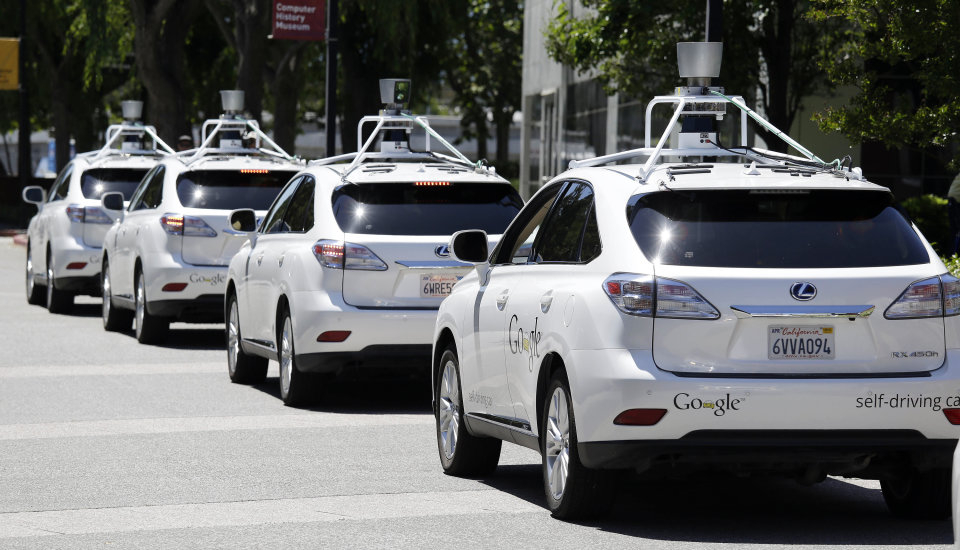
\includegraphics[height=3cm]{google-selfdriving-cars}
        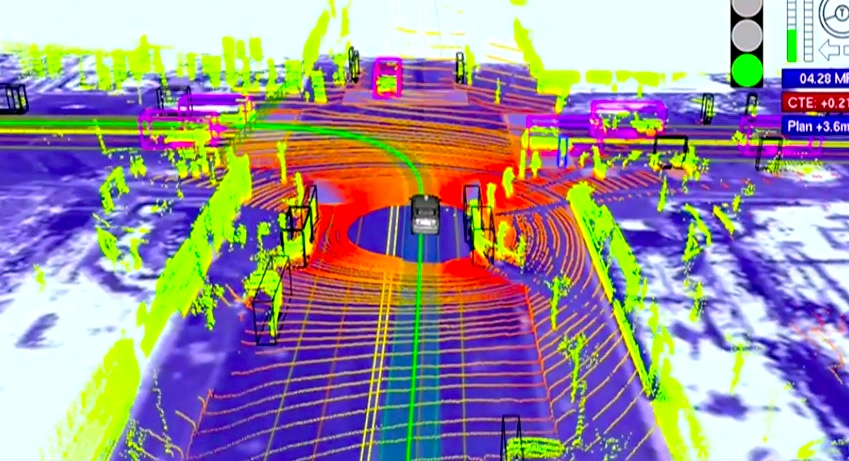
\includegraphics[height=3cm]{google-selfdriving-cars-3dview}

        \source{https://www.engadget.com/2015/07/07/google-self-driving-tests-austin-texas/}{Engadget}
        \hspace{15em}
        \source{http://spectrum.ieee.org/automaton/robotics/artificial-intelligence/how-google-self-driving-car-works}{IEEE Spectrum}

    24 Lexus + 34 'Google Cars'; between 2009 and August 2016, autonomously driven $\approx$ 2 000 000 miles
}
    \only<4>{

        \textbf{Uber autonomous taxis} 

        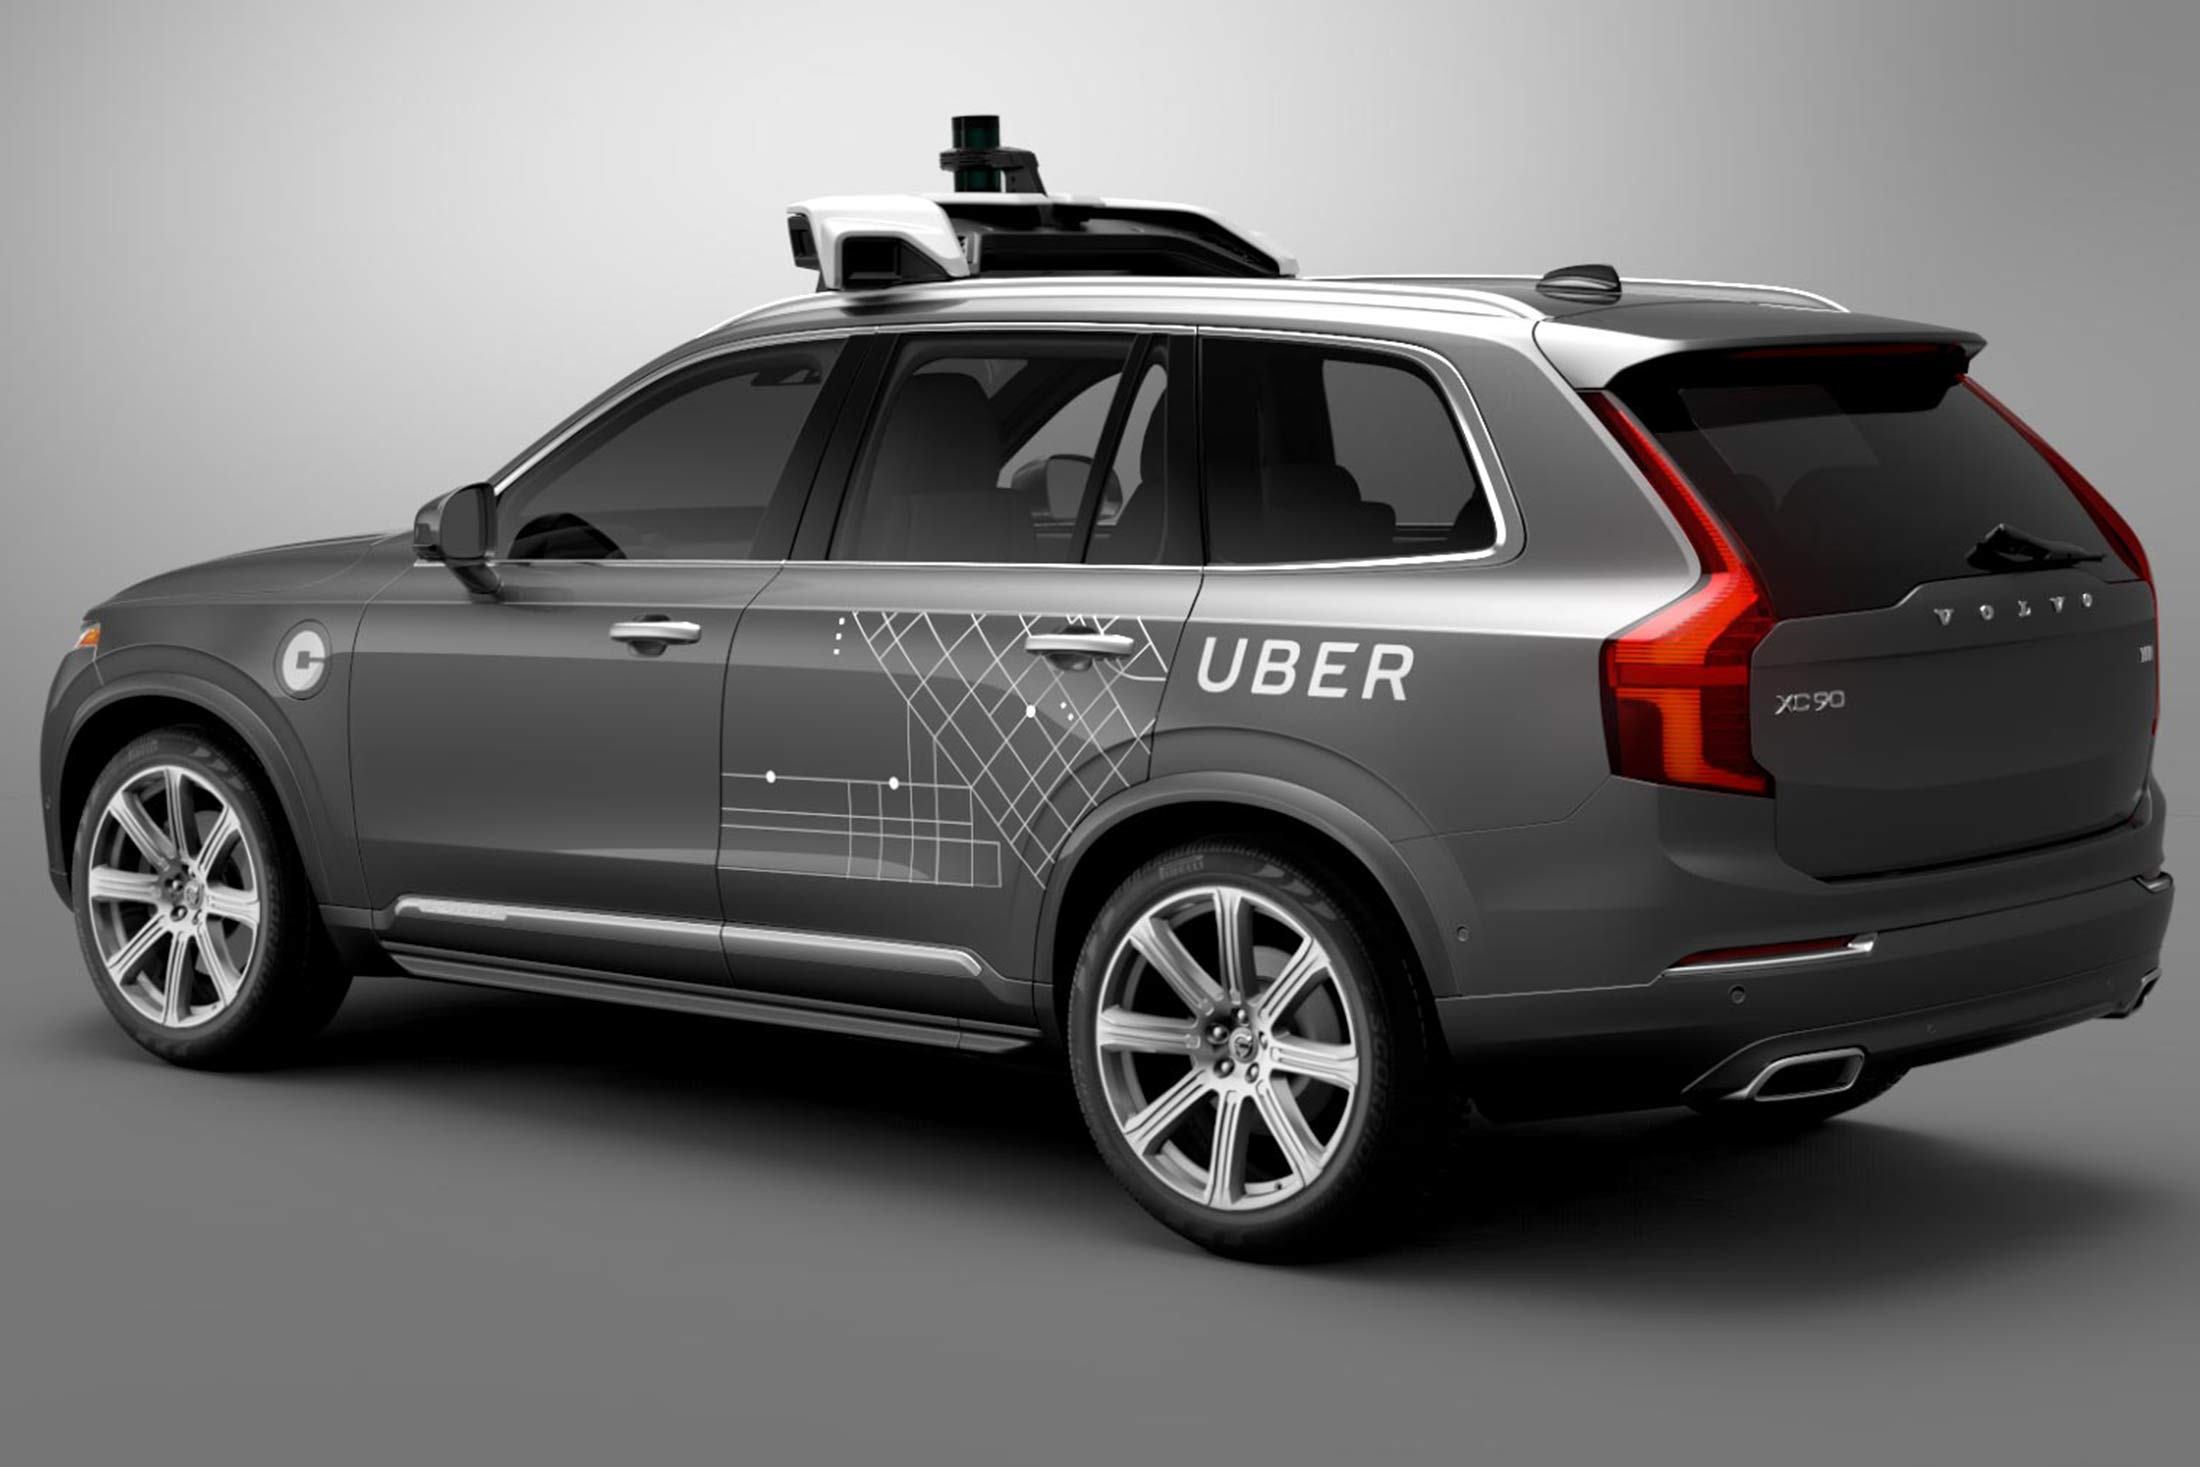
\includegraphics[width=0.7\linewidth]{uber-autonomous-cars}

        \source{http://www.bloomberg.com/news/features/2016-08-18/uber-s-first-self-driving-fleet-arrives-in-pittsburgh-this-month-is06r7on}{Bloomberg}

        100 Volvo cars ...already driving in Pittsburg's streets! (with human supervision)

}



%
%Video
%
%\begin{itemize}
%\item
%  \href{http://youtu.be/M2AcMnfzpNg}{Overview of 2nd DARPA Grand
%  Challenge 2005}
%\item
%  \href{http://youtu.be/cdgQpa1pUUE}{Google Car promo video}
%\end{itemize}

\end{frame}

{\fullbackground{nao}

\begin{frame}{Humanoids}

Human-like robots.

Tremendously challenging:

    \begin{itemize}
        \item Power, 
        \item actuations, 
        \item artificial intelligence, 
        \item perception, 
        \item control,
        \item walking, \ldots{}
    \end{itemize}


\begin{itemize}
\item
  \href{http://youtu.be/yND4k4NM0qU}{Honda Asimo latest version}
\item
  \href{http://youtu.be/aqCmX5dMYHg}{Boston Dynamics Petman prototype}
  and \href{http://youtu.be/FFGfq0pRczY}{obstacle negotiation}.
\item
  \href{https://www.youtube.com/watch?v=g0TaYhjpOfo}{DARPA Robotics
  challenge 2015 outtakes}
\end{itemize}

\end{frame}
}

\begin{frame}{And what do I do?}

\begin{multicols}{2}

    \textbf{Cognitive robotics}

  Building robots and their artificial intelligence inspired on natural
  systems, such as developing children

    \textbf{Human-Robot Interaction}

  Building robots that can work alongside people, using social cues that
  people use to communicate

    \begin{center}
        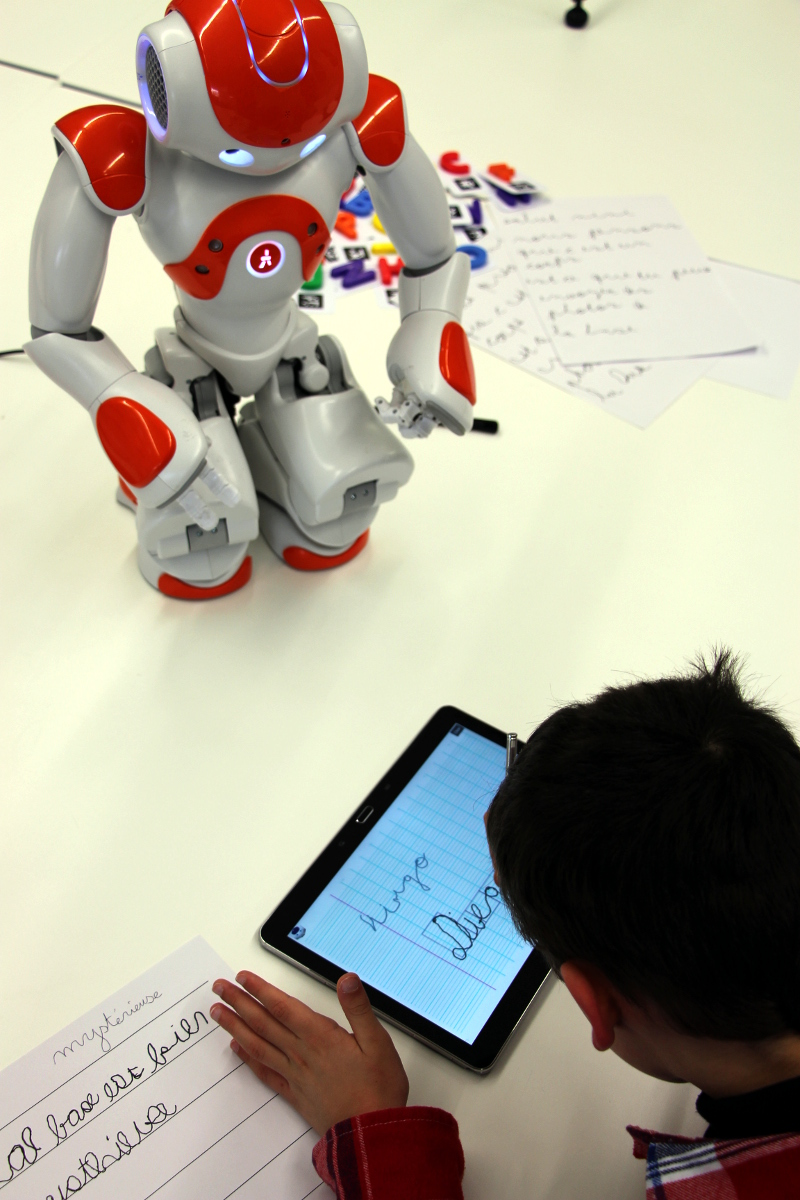
\includegraphics[width=0.8\linewidth]{cowriter}
    \end{center}

\end{multicols}
\end{frame}


\begin{frame}{}
    \begin{center}
        \Large
        That's all, folks!\\[2em]
        \normalsize
        See you on Friday, 13:00, for the first lab\\[1em]
        Questions:\\
        Portland Square A216 or \url{severin.lemaignan@plymouth.ac.uk} \\[1em]

        Slides:\\ \href{https://github.com/severin-lemaignan/module-mobile-and-humanoid-robots}{\small github.com/severin-lemaignan/module-mobile-and-humanoid-robots}

    \end{center}
\end{frame}



\end{document}
